\chapter{Marco te\'orico}

\section{PBR}
PBR o \textit{physically based rendering} es el t\'ermino que se utiliza para nombrar al grupo de t\'ecnicas basados en un
modelo f\'isico. La intenci\'on es conseguir aproximaciones r\'apidas y plausibles de la interacci\'on de un flujo de luz
con una superficie. Las principales ventajas de este tipo de algoritmos son la consistencia bajo diferentes condiciones de
luz y su manejo intuitivo por parte de los artistas.
Los motores PBR cumplen con la ley de la conservaci\'on de la energ\'ia y utilizan BRDFs basados en la teor\'ia de
microfacetas. Adicionalmente, otros elementos de la escena, como la c\'amara o las luces, pueden estar basados en modelos
f\'isicos para ofreciendo para aumentar el grado de realismo.

\section{Ecuaci\'on de render}
El prop\'osito de la ecuacion de render es conocer el valor de radiancia que llega a la camara en una direcci\'on
por cada pixel  de la camara.

Para saber la radiancia sobre un punto en una direcci\'on, utilizamos la ecuacion de reflectancia, que depende
de la luz que llega al puntos, el coseno del angulo con el que incide la luz y el BRDF (bidirectional reflectance
distribution function), que modela el comportamiento de la luz al rebotar sobre la superficie.

\begin{equation}
L_o(p, w_o) = L_e(x, w_o) + \int_\Omega{f_r(p, w_i, w_o) L_i(p, w_i) n\cdot{w_i}dw_i}
\end{equation}


Siendo $L_o(p, w_o)$ la luz reflectada por la superficie, $L_e(x, w_o)$ la luz emitida por la superficie, que est\'a fuera
de la integral porque es independiente de la luz reflejada o refractada por la superficie. $\int_{\Omega}[...]dw\int_{\Omega}
[...]dw$ que representa que la operaci\'on se repite para cada \'angulo s\'olido dentro de la semiesfera $f_r(p, w_i, w_o)$ el
BRDF $L_i(p, w_i)$ la luz que llega al punto de la superficie que estamos evaluando $n\cdot{w_i}$ el factor de atenuaci\'on
de la luz con respecto a la normal.

\section{BRDF}

El BRDF, o función de ditribuci\'on bidireccional de reflectividad, es la parte de la ecuaci\'on que describe el
comportamiento de la luz al golpear sobre la superficie y se utiliza para rmodelar propiedades f\'isicas de los diferentes
materiales. Es una funcion estad\'istica que calcula cuanta de la luz que incide sobre un material es reflejada en direcci\'on
a la c\'amara, o, en otras palabras, para ello toma como argumentos la direccion de la luz, $w_i$, y la dirección de salida,
$w_o$, la normal de la superficie, n, y un par\'ametro $\alpha$ que representa la rugosidad del material.

\begin{figure}[H]
    \vspace{0.5cm}
    \centering
      \frame{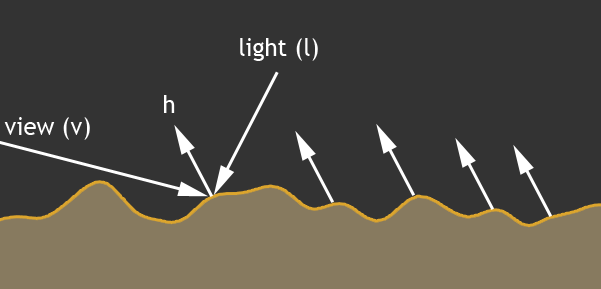
\includegraphics[scale=0.7]{microfacet-diagram}}
    \caption{Diagrama de la luz incidente y luz reflectada}
    \vspace{0.5cm}
\end{figure}

Para que un BRDF se considere como PBR, ha de utilizar el modelo de microfacetas, ademas de cumplir con la ley de conservacion
de la energia, $\forall w_i \int_{\Omega} f(p, w_i, w_o) n\cdot{w_i} dw_o \leq 1$ y el principio de reciprocidad de Helmholtz,
el BRDF debe de ser simétrico, esto es que invertir la direccion de entrada y salida del BRDF no deberia afectar al resultado
$f(x, w_i, w_o) = f(x, w_o, w_i)$ sin embargo, los motores en tiempo real, frecuentemente incumplen el principio de reciprocidad,
no siendo fisicamente plausibles, pero sin generar artefactos.\\

    \subsection{Teor\'ia de microfacetas}

    \bgroup

        Aunque a nivel macrosc\'opico podamos considerar una superficie como lisa, ninguna superficie es completamente lisa a nivel
        microsc\'opico. La teor\'ia de microfacetas utiliza una representaci\'on estad\'istica para modelar estas peque\~nas irregularidades.
        Para ello, la teor\'ia de microfacetas, considera la superficie de reflexi\'on como una superficie compuesta por una matriz de
        superficies mas pequenhas que la longitud de onda de la luz pero muy peque\~nas desde el punto de vista de la c\'amara,
        completamente reflectantes, llamadas microfacetas, y cuyas diferentes orientaciones determinan la rugosidad de la superficie.
        Si las microfacetas est\'an completamente alineadas, las reflexiones ser\'an mas definidas, asimilandose a un espejo, mientras
        que las microfacetas apuntando en diferentes direcciones, daran como resultado una reflexion especular mas difusa.

        \begin{figure}[H]
            \vspace{0.5cm}
            \centering
            \frame{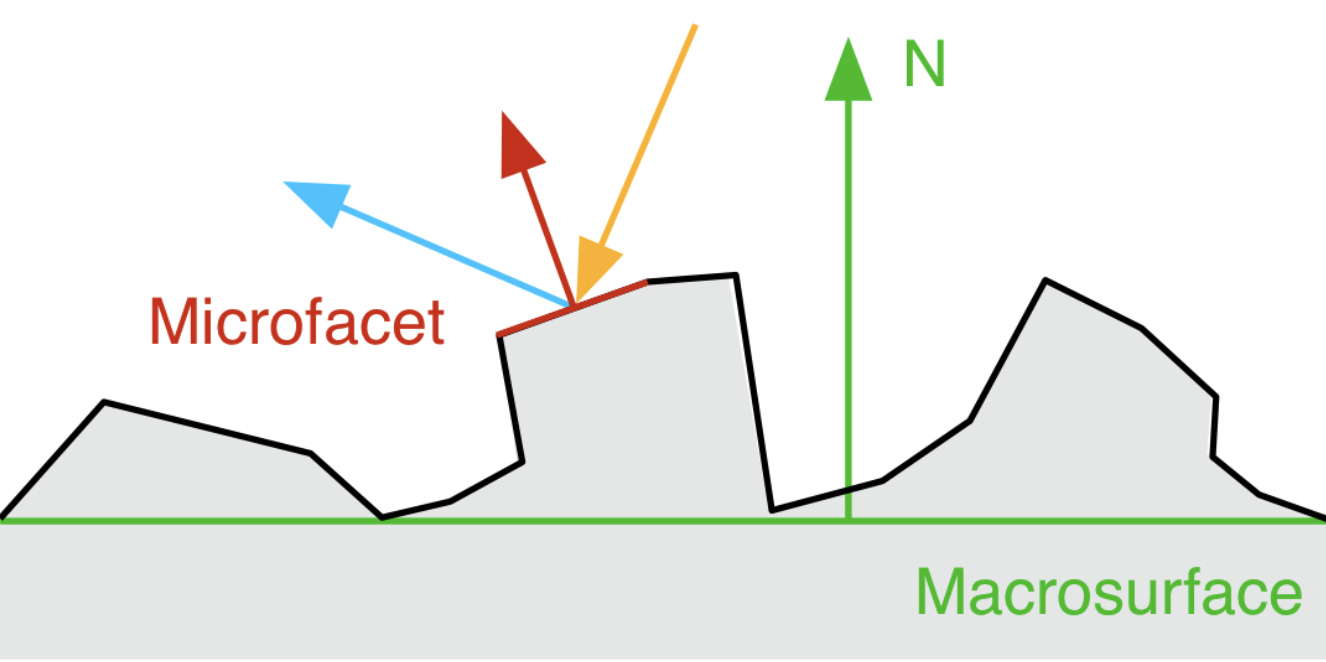
\includegraphics[scale=0.55]{macrosuperficie}}
            \caption{Superficie a escala microsc\'opica}
            \vspace{1.0cm}
        \end{figure}

    \egroup


    \subsection{Tipos de BRDFs}
    Los diferentes tipos de BRDFs permiten para modelar diferentes propiedades de los materiales, isotropia o anisotropia,
    transmitancia, reflexiones internas, etc. Podemos clasificar los diferentes tipos de BRDFs entre modelos analiticos y BDRFs
    de datos adquiridos. Los modelos analiticos son funciones matemáticas que modelan diferentes efectos de la luz en funcion de
    sus datos de entrada, mientras que los BRDFs de datos adquiridos, capturan el BRDF de un material con un gonioreflectometro,
    y permiten una representacion muy precisa del material escaneado.

    \begin{figure}[H]
        \vspace{0.5cm}
        \centering
        \frame{\includegraphics[scale=0.6]{MERL}}
        \caption{MERL}
        \vspace{0.5cm}
    \end{figure}

    Comunmente, en la industria se utilizan modelos analiticos, debido a su flexibilidad y rendicimiente y el mas utilizado a
    dia de hoy en la industria, aunque con algunas variaciones en sus terminos, sigue siendo el modelo de Cook-Torrance.

    \subsection{Modelo de Cook-Torrance}
        Es un modelo anal\'itico permite representar con gran realismo materiales electricos y dielectricos con diferentes
        grados de rugosidad y, en general, funciona bien para modelar cambios en el color que dependen del punto de vista.\\
        Este modelo permite estudiar por separado las dos componentes de la luz, especular y difuso:

        \begin{equation}
        f_r = k_{d}f_{lambert} + k_sf_{cook-torrance}
        \end{equation}
        
        siendo $k_d$ y $k_s$, parametros de peso:

        \begin{equation}
        k_d + k_s = 1
        \end{equation}

        Tipicamente la componente difusa, utiliza el modelo de Lambert, que asume una distribución completamente uniforme a lo
        largo de la superficie:

        \begin{equation}
        f_{Lambert} = \frac{diffuse}{\pi}
        \end{equation}

        La componente especular es una funci\'on compuesta de otras tres funciones y un factor de normalizaci\'on en el
        denominador.

        \begin{equation}
            f(l, v) = \frac{F(w_i, h) G(w_i, h, w_o) D(h)} {4(n\cdot{w_i}) (n \cdot{w_o})}
        \end{equation}

    \subsection{T\'erminos del BRDF}
        El BRDF de Cook-Torrance est\'a compuesto por otras tres funciones y un factor de normalizaci\'on en el denominador.
        Las funciones D, F y G, se corresponden con la funci\'on de distribuci\'on de las normales, la ecuaci\'on de Fresnel,
        y la funci\'on de geometr\'ia.\\

        $D(l, v, h)$  es la funci\'on de distribuci\'on de las normales y se encarga de representar la rugosidad de una superficie
        y es el t\'ermino que afecta en mayor grado a la forma y taman\~no del brillo especular. T\'ipicamente el par\'ametro
        \textit{roughness} se utiliza para representar la cantidad de microfacetas alineadas con la normal h, cuanta mayor sea la
        la cantidad de de microfacetas alineadas, m\'as lisa parecer\'a la superficie.

        $$
        D(h) = \frac{\alpha^2}{\pi((n\cdot{h})^2(\alpha^2 - 1) + 1)^2}
        $$

        \begin{figure}[H]
            \vspace{0.5cm}
            \centering
              \frame{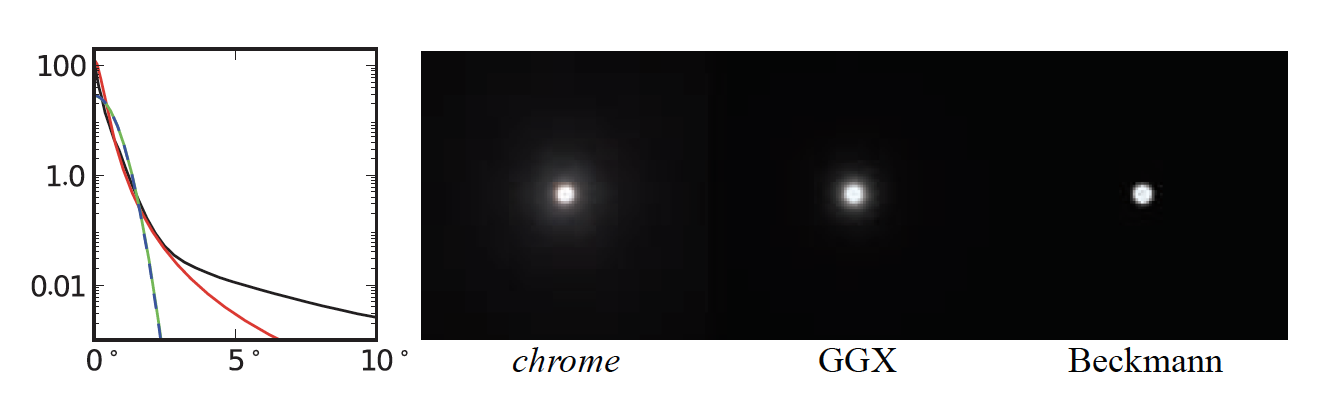
\includegraphics[scale=0.65]{ndf}}
            \caption{Representaci\'on gr\'afica de la funci\'on de geometr\'ia}
        \end{figure}

        $G(w_o)$ es la funci\'on de gromatr\'ia. \'Esta funci\'on tiene en cuenta las oclusiones de la superficie.
        Mientras que el t\'ermino de distribucion de las normales, D(h), define la concentraci\'on de microfacetas con una normal h,
        no define si esas microfacetas son visible o no. El t\'ermino de geometr\'ia tiene en cuenta las dos cosas, la sombra
        y el enmascaramiento. La sombra representa que una microfaceta no es visible desde la direcci\'on de la luz, mientras que el
        enmascaramiento significa que una microfaceta no es visible desde la direcci\'on de vista y, por tanto, no contribuyen
        a la reflexi\'on.

        $$
        G(w_i, w_o, h) = G(w_i)G(w_o)
        $$

        $$
        G(w_o) = \frac{n\cdot{w_o}}{(n\cdot) (1 - k) + k}
        $$

        $$
        k = \frac{(roughness + 1)^2}{8}
        $$

        \begin{figure}[H]
            \vspace{0.5cm}
            \centering
              \frame{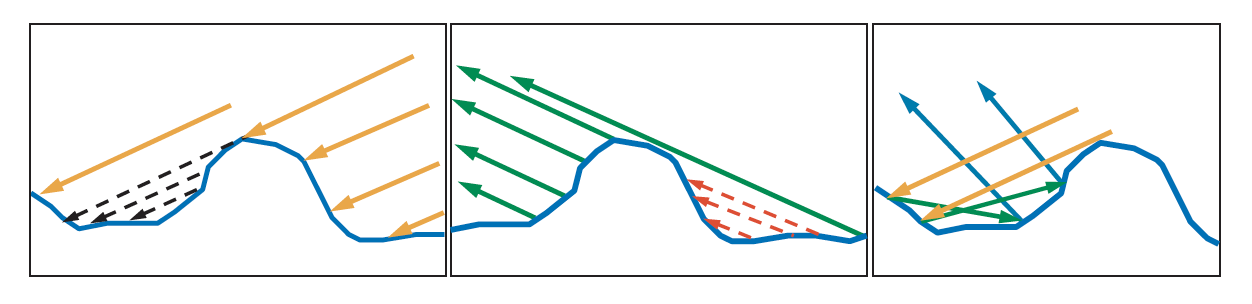
\includegraphics[scale=0.65]{microgeometria}}
            \caption{Representaci\'on gr\'afica de la sombra y el enmascaramiento en la funci\'on de geometr\'ia}
        \end{figure}

        $F(l, v, h)$ es la funci\'on de Fresnel. Representa la radiancia reflejada por un material seg\'un el \'angulo de incidencia
        de la luz. Para la mayor\'ia de los materiales no met\'alicos, las reflexiones son m\'as intensas bajo cuando el \'angulo
        de incidencia es muy agudo. En la mayor\'ia de los algoritmos de sombreado, el fresnel se utiliza a nivel de la macrosuperficie,
        sin embargo, al aplicar el fresnel sobre la normal de la microfacetas, se consigue un mayor grado de realismo para los valores
        altos de \textit{roughness}.

        $$
        F_{Schlick}(F_o, w_i, h) = F_o + (1 - F_o) (1 - (l\cdot{h}))^5
        $$
    
        \begin{figure}[H]
            \vspace{0.5cm}
            \centering
              \frame{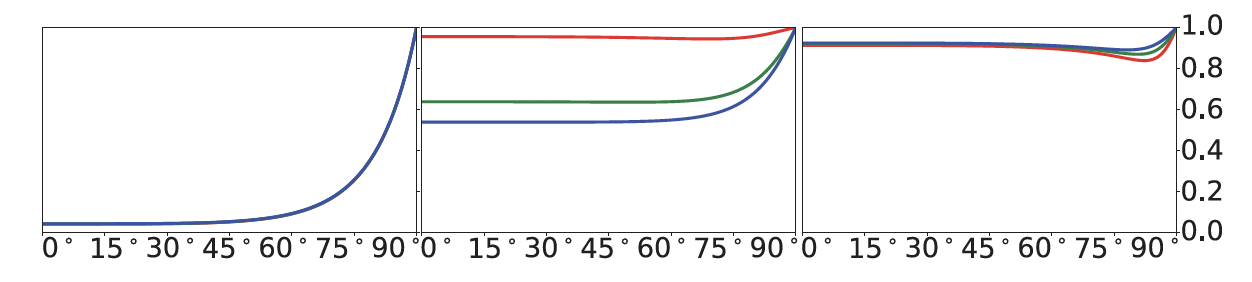
\includegraphics[scale=0.65]{fresnel}}
            \caption{Representaci\'on gr\'afica de la funci\'on de geometr\'ia}
        \end{figure}

        \todo[inline]{Hablar del denominador}

        % La funci\on de distribuci\'on de las normales, aproxima la cantidad de microfacetas aproxima la alineadas con el
        % vector h, el medio entre el rayo de luz y el punto del vista. El par\'ametro que modela la rugosidad de una superficie
        % afecta en gran medida al resultado. Este es el factor m\'as caracter\'istico del modelo de microfacetas.
        % La funci\'on de geometr\'ia describe la cantidad de rayos ocluidos por las propias microfacetas.\\

        % Finalmente, la ecuaci\'on de fresnel describe el ratio de reflexi\'on de una superficie bajo diferentes \'angulos de
        % incidencia.\\

\section{Disney Principled BRDF}

El BRDF de Disney fue presentado por Brent Burley en 2012 y es el utilizado por Disney en sus peliculas de animacion. Es,
junto al modelo de Cook-Torrance, el mas utilizado en los motores de tiempo real, sin embargo, el modelo de Burley, es mas
amigable para los artistas, a costa de no ser completamente basado en fisica. Los parametros tienen nombres y valores que
definen que el aspecto de los materiales son mas intuitivos. Los lobulos adicionales, a diferencia del modelo de Cook-Torrance,
pueden variar mucho en forma y tamanho, por lo que es un modelo muy flexible, que permite representar con gran realismo una
amplia variedad de materiales.\\

\begin{figure}[H]
    \vspace{0.5cm}
    \centering
      \frame{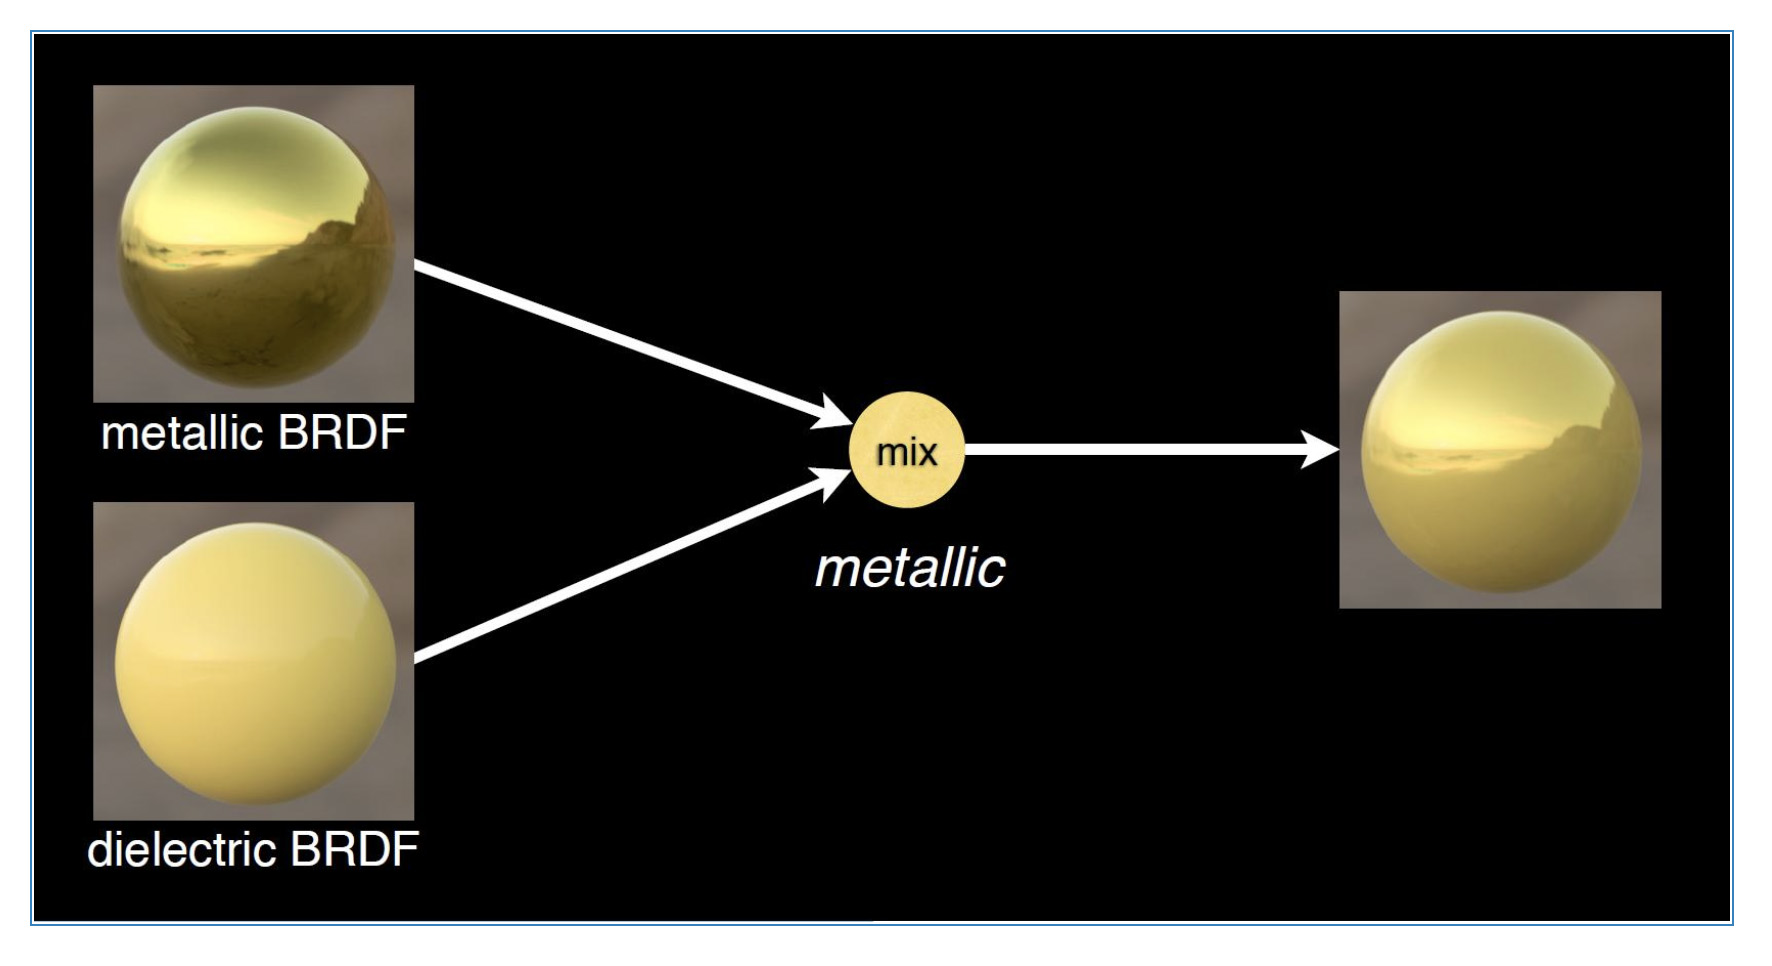
\includegraphics[scale=0.47]{disney}}
    \caption{Modelo de Disney}
\end{figure}

Es conocido como \textit{principled} por cumplir una serie de maximas, que se respetan en el modelo por encima de las leyes fisicas.
El modelo ha de ser intuitivo y no utilizar parametros que se refieran al modelo basado en fisica, debe tener el menor
numero de parametros posible, deben de estar normalizados, algunos valores pueden exceder su rango para permitir mayor
expresividad y, finalmente, todas las combinaciones de parametros deben de ser robustas y plausibles. Para ello utiliza los
siguientes par\'ametros:

\begin{itemize}
	\item baseColor: el color de la superficie, comunmente utiliza un mapa.
	\item subsurface: aproximacion para controlar el color de la reflexion difusa.
	\item metal interpolaci\'on lineal entre los dos modelos. El met\'alico no tiene
    componente de reflexi\'on difusa y su componente de reflexi\'on especular es del mismo color que el color base. 
    \item specular: cantidad de luz incidente reflejada, se utiliza para controlar de forma intuitiva el \'indice de refracci\'on de
    una superficie.
	\item specularTint: par\'ametro que permite a los artistas controlar el color de la reflexi\'on especular sobre el color
	base.
	\item roughness: describe la rugosidad de una superficie, afectando a la reflexi\'on difusa y especular.
	\item sheen: ermite mayor grado de control sobre la reflexi\'on especular, muy \'util sobre tejidos.
	\item sheenTint: color del \textit{sheen}
	\item clearCoat: un l\'obulo extra.
	\item clearcoatGloss: permite controlar la rugosidad de este l\'obulo.
\end{itemize}
    
    \subsection{Componente difusa}

    En base a las observaciones sobre los datos de MERL, el modelo difuso parece muy oscuro hacia los bordes, y aplicando
    la funci\'on de Fresnel, para intentar conseguir un modelo f\'isicamente plausible, parece oscurecer m\'as los bordes,
    acentuando el problema. Disney desarroll\'o un modelo emp\'irico, que utiliza la aproximaci\'on de Fresnel Schlick:

    $$
    (1 - F(\theta_l) (1 - F(\theta_d)))
    $$

    Modificandolo para conseguir que la retroreflexi\'on dependa del valor de \textit{roughness} y as\'i
    adaptarse mejor a los datos obtenidos de MERL.

    $$
    f_d = \frac{baseColor}{\pi}
    \left(  1 + (F_{D90} - 1)(1 - cos\theta_{wi})^5  \right)
    \left(  1 + (F_{D90} - 1)(1 - cos\theta_{wo})^5  \right)
    $$
    
    $$
    F_{D90} = 0.5 + 2roughness\cdot{cos^2\theta_d}
    $$

    \subsection{Componente especular}
        \subsection{F, t\'ermino de Fresnel}
        Para el especular, la aproximaci\'on de Fresnel Schlick es lo suficientemente precisa y mucho menos costosa que
        que la ecuaci\'on completa de Fresnel.

        $$
        (1 - F(\theta_l) (1 - F(\theta_d)))^5
        $$

        $F_0$ representa la reflectancia de una incidencia del mismo \'angulo que la normal. $\theta_d$ es el \'angulo
        entre el vector $h$, y el de vista $w_o$.

        \subsubsection{G, t\'ermino de geometr\'ia}
        En el t\'ermino G, Disney utiliza dos modelos diferentes, uno para el l\'obulo primario y otro para el de clearcoat.
        Para el l\'obulo primario, utiliza el modelo de Smith GGX, remapeando el valor de \textit{roughness} para evitar
        ganar demasiada energ\'ia hacia los bordes de materiales brillantes.

        $$
        G_{GGX}(v) = \frac
        {2 (n \cdot{v})}
        {(n \cdot{v}) + \sqrt{ \alpha^2 + (1 - \alpha)^2 (n \cdot{v})^2 }}
        $$

        $$
        G(l, v, h) = G_{GGX}(l)G_{GGX}(v)
        $$

        $$
        \alpha = (0.5 + roughness / 2)^2
        $$

        \subsubsection{D, t\'ermino de distribuci\'on de las normales}
        

